% Competitive Programming Bootcamp Day 0
% Compile with: pdflatex day0_slides.tex
% No shell-escape required.

\documentclass[aspectratio=169,11pt]{beamer}

% ------------------------------------------------------------
% Packages
% ------------------------------------------------------------
\usepackage[utf8]{inputenc}
\usepackage[T1]{fontenc}
\usepackage{lmodern}
\usepackage{amsmath,amssymb,mathtools}
\usepackage{booktabs}
\usepackage{array}
\usepackage{xcolor}
\usepackage{tikz}
\usepackage{hyperref}
\usetikzlibrary{arrows.meta,positioning,shapes.geometric}

% ------------------------------------------------------------
% Theme setup
% ------------------------------------------------------------
\definecolor{CPNavy}{HTML}{172033}
\definecolor{CPBlue}{HTML}{2563EB}
\definecolor{CPGreen}{HTML}{16A34A}
\definecolor{CPOrange}{HTML}{F97316}
\definecolor{CPRed}{HTML}{DC2626}
\definecolor{CPGray}{HTML}{64748B}
\definecolor{CPLight}{HTML}{F8FAFC}
\definecolor{CPCodeBg}{HTML}{F1F5F9}

\usetheme{default}
\usefonttheme{professionalfonts}
\setbeamertemplate{navigation symbols}{}
\setbeamertemplate{itemize item}{\color{CPBlue}$\blacktriangleright$}
\setbeamertemplate{itemize subitem}{\color{CPGray}$\triangleright$}
\setbeamertemplate{enumerate item}{\color{CPBlue}\insertenumlabel.}

\setbeamercolor{normal text}{fg=CPNavy,bg=white}
\setbeamercolor{frametitle}{fg=white,bg=CPNavy}
\setbeamercolor{title}{fg=white,bg=CPNavy}
\setbeamercolor{subtitle}{fg=CPLight,bg=CPNavy}
\setbeamercolor{block title}{fg=white,bg=CPBlue}
\setbeamercolor{block body}{fg=CPNavy,bg=CPLight}
\setbeamercolor{alerted text}{fg=CPRed}

% Frame title bar
\setbeamertemplate{frametitle}{%
  \nointerlineskip%
  \begin{beamercolorbox}[wd=\paperwidth,ht=0.92cm,dp=0.25cm,leftskip=0.55cm,rightskip=0.4cm]{frametitle}
    \usebeamerfont{frametitle}\insertframetitle\hfill\small\insertframenumber/\inserttotalframenumber
  \end{beamercolorbox}%
}

% Title page
\setbeamertemplate{title page}{%
  \begin{tikzpicture}[remember picture,overlay]
    \fill[CPNavy] (current page.south west) rectangle (current page.north east);
    \fill[CPBlue] ([xshift=-1.4cm,yshift=-1.2cm]current page.north east) circle (2.7cm);
    \fill[CPOrange] ([xshift=0.6cm,yshift=0.2cm]current page.south west) circle (2.2cm);
  \end{tikzpicture}
  \vspace{1.2cm}
  {\color{white}\Huge\bfseries\inserttitle\par}
  \vspace{0.3cm}
  {\color{CPLight}\Large\insertsubtitle\par}
  \vfill
  {\color{CPLight}\large\insertauthor\par}
  \vspace{0.1cm}
  {\color{CPLight}\insertdate\par}
}

% Footer
\setbeamertemplate{footline}{%
  \leavevmode%
  \hbox{%
    \begin{beamercolorbox}[wd=.5\paperwidth,ht=2.4ex,dp=1ex,leftskip=.5cm]{author in head/foot}%
      \color{CPGray}\insertshorttitle
    \end{beamercolorbox}%
    \begin{beamercolorbox}[wd=.5\paperwidth,ht=2.4ex,dp=1ex,rightskip=.5cm plus1fil]{date in head/foot}%
      \hfill\color{CPGray}\insertshortauthor
    \end{beamercolorbox}%
  }%
}

% ------------------------------------------------------------
% Reusable slide helpers
% ------------------------------------------------------------
\newenvironment{cpbox}[1]{%
  \begin{block}{#1}
  }{%
  \end{block}
}

\newcommand{\rulecard}[2]{%
  \begin{cpbox}{#1}
    #2
  \end{cpbox}
}

% ------------------------------------------------------------
% Deck metadata
% ------------------------------------------------------------
\title[CP Bootcamp]{Competitive Programming Bootcamp Day 0}
\subtitle{ICPC Orientation, Rules, Skills, and Team Building}
\author[Ryan Pelchat]{Ryan Pelchat}
\date{August 2026}

\begin{document}

% ------------------------------------------------------------
\begin{frame}[plain]
  \titlepage
\end{frame}

% ------------------------------------------------------------
\begin{frame}{Today's Roadmap}
  \begin{enumerate}
    \item What ICPC is and why we train for it
    \item Core ICPC-style contest rules
    \item Skills needed to perform under contest pressure
    \item Team building and icebreaker activity
    \item Day 0 outcomes and next steps
  \end{enumerate}
\end{frame}

% ------------------------------------------------------------
\begin{frame}{What Is ICPC?}
  \begin{itemize}
    \item ICPC stands for the International Collegiate Programming Contest.
    \item It is a university-level, team-based programming contest.
    \item Teams solve algorithmic problems by writing code that is judged automatically.
    \item The contest rewards problem solving, programming fluency, teamwork, and calm execution.
  \end{itemize}

  \vspace{0.35cm}
  \begin{cpbox}{Day 0 framing}
    ICPC is not only about knowing algorithms. It is about turning ideas into accepted submissions with limited time, shared equipment, and teammates depending on each other.
  \end{cpbox}
\end{frame}

% ------------------------------------------------------------
\begin{frame}{What Makes ICPC Different?}
  \begin{center}
    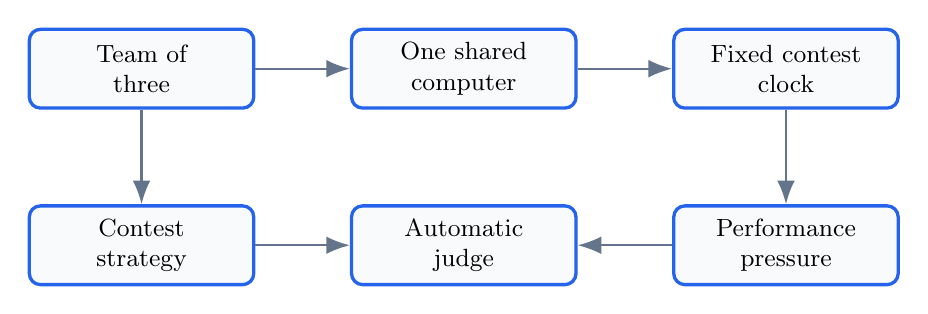
\begin{tikzpicture}[
        node distance=1.2cm,
        every node/.style={font=\small},
        box/.style={rounded corners,draw=CPBlue,very thick,align=center,minimum width=2.85cm,minimum height=1.0cm,fill=CPLight},
        arrow/.style={-{Latex[length=3mm]},thick,draw=CPGray}
      ]
      \node[box] (team) {Team of\\three};
      \node[box,right=of team] (computer) {One shared\\computer};
      \node[box,right=of computer] (clock) {Fixed contest\\clock};
      \node[box,below=of computer] (judge) {Automatic\\judge};
      \node[box,left=of judge] (strategy) {Contest\\strategy};
      \node[box,right=of judge] (pressure) {Performance\\pressure};

      \draw[arrow] (team) -- (computer);
      \draw[arrow] (computer) -- (clock);
      \draw[arrow] (team) -- (strategy);
      \draw[arrow] (clock) -- (pressure);
      \draw[arrow] (strategy) -- (judge);
      \draw[arrow] (pressure) -- (judge);
    \end{tikzpicture}
  \end{center}
\end{frame}

% ------------------------------------------------------------
\begin{frame}{The Contest Loop}
  \begin{center}
    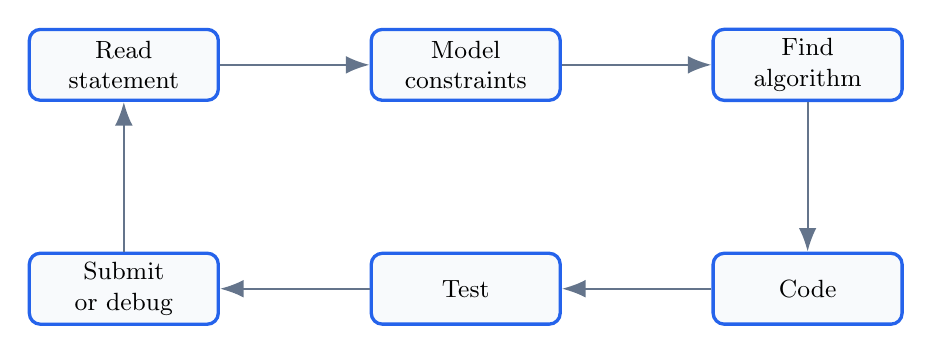
\begin{tikzpicture}[
        node distance=1.9cm,
        every node/.style={font=\small},
        box/.style={rounded corners,draw=CPBlue,very thick,align=center,minimum width=2.4cm,minimum height=0.9cm,fill=CPLight},
        arrow/.style={-{Latex[length=3mm]},thick,draw=CPGray}
      ]
      \node[box] (read) {Read\\statement};
      \node[box,right=of read] (model) {Model\\constraints};
      \node[box,right=of model] (solve) {Find\\algorithm};
      \node[box,below=of solve] (code) {Code};
      \node[box,left=of code] (test) {Test};
      \node[box,left=of test] (submit) {Submit\\or debug};

      \draw[arrow] (read) -- (model);
      \draw[arrow] (model) -- (solve);
      \draw[arrow] (solve) -- (code);
      \draw[arrow] (code) -- (test);
      \draw[arrow] (test) -- (submit);
      \draw[arrow] (submit) -- (read);
    \end{tikzpicture}
  \end{center}
\end{frame}

% ------------------------------------------------------------
\begin{frame}{Typical ICPC-Style Format}
  \begin{columns}[T,onlytextwidth]
    \column{0.5\textwidth}
      \rulecard{Team Setup}{
        \begin{itemize}
          \item Three contestants per team
          \item One shared workstation
          \item Communication only within the team and contest staff
        \end{itemize}
      }

    \column{0.5\textwidth}
      \rulecard{Problem Set}{
        \begin{itemize}
          \item Several algorithmic problems
          \item Usually around five hours
          \item Submissions judged as accepted or rejected
        \end{itemize}
      }
  \end{columns}

  \vspace{0.25cm}
  \begin{cpbox}{Important}
    Exact eligibility, languages, printed materials, environment, and site rules are published by each official contest. Always check the current regional rules before competing.
  \end{cpbox}
\end{frame}

% ------------------------------------------------------------
\begin{frame}{Scoring and Ranking}
  \begin{itemize}
    \item Teams are ranked first by the number of accepted problems.
    \item Ties are usually ranked by lower total penalty time.
    \item For each solved problem, penalty includes the accepted submission time.
    \item Rejected attempts before the accepted run usually add 20 minutes each.
    \item Unsolved problems do not add time penalty.
    \item Compile errors are commonly not counted as 20-minute penalties, but always confirm local rules.
  \end{itemize}
\end{frame}

% ------------------------------------------------------------
\begin{frame}{Scoring Example}
  \begin{center}
  \small
  \begin{tabular}{@{}lccc@{}}
    \toprule
    Problem & Result & Attempts Before AC & Score Impact \\
    \midrule
    A & Accepted at 18 min & 0 & 18 \\
    B & Accepted at 73 min & 2 & 73 + 40 = 113 \\
    C & Unsolved & 5 & 0 \\
    \midrule
    Total & 2 solved & & 131 penalty \\
    \bottomrule
  \end{tabular}
  \end{center}

  \vspace{0.35cm}
  \begin{cpbox}{Strategy lesson}
    Wrong submissions matter only when the problem is eventually solved, but repeated guessing can still waste the contest clock and slow the team.
  \end{cpbox}
\end{frame}

% ------------------------------------------------------------
\begin{frame}{Contest Conduct}
  \begin{columns}[T,onlytextwidth]
    \column{0.5\textwidth}
      \begin{cpbox}{Allowed During Contest}
        \begin{itemize}
          \item Team discussion
          \item Approved programming environment
          \item Contest system submissions
          \item Clarification requests to judges
        \end{itemize}
      \end{cpbox}

    \column{0.5\textwidth}
      \begin{cpbox}{Generally Not Allowed}
        \begin{itemize}
          \item Outside communication
          \item Unapproved websites or remote access
          \item Unauthorized electronic devices
          \item Tools that contact external services
        \end{itemize}
      \end{cpbox}
  \end{columns}

  \vspace{0.25cm}
  \begin{cpbox}{When unsure}
    Ask a judge or proctor. In contest settings, guessing about rules is a bad risk.
  \end{cpbox}
\end{frame}

% ------------------------------------------------------------
\begin{frame}{Skills Needed to Perform}
  \begin{center}
  \small
  \begin{tabular}{@{}ll@{}}
    \toprule
    Skill Area & What It Looks Like in Contest \\
    \midrule
    Problem reading & Identify input, output, constraints, edge cases \\
    Algorithm design & Match patterns to correct complexity \\
    Implementation & Write reliable code quickly \\
    Testing & Build small, adversarial, and boundary cases \\
    Debugging & Isolate mistakes without panic \\
    Strategy & Choose which problem deserves time now \\
    Teamwork & Communicate clearly around one computer \\
    \bottomrule
  \end{tabular}
  \end{center}
\end{frame}

% ------------------------------------------------------------
\begin{frame}{Technical Skill Stack}
  \begin{columns}[T,onlytextwidth]
    \column{0.34\textwidth}
      \rulecard{Fluency}{
        \begin{itemize}
          \item Language basics
          \item Standard library
          \item Fast input/output
          \item Templates
        \end{itemize}
      }

    \column{0.33\textwidth}
      \rulecard{Algorithms}{
        \begin{itemize}
          \item Sorting and search
          \item Graph traversal
          \item Greedy methods
          \item Dynamic programming
        \end{itemize}
      }

    \column{0.33\textwidth}
      \rulecard{Judgment}{
        \begin{itemize}
          \item Complexity bounds
          \item Proof idea
          \item Edge cases
          \item Failure modes
        \end{itemize}
      }
  \end{columns}
\end{frame}

% ------------------------------------------------------------
\begin{frame}{Team Skill Stack}
  \begin{itemize}
    \item \textbf{Driver:} types the solution and explains implementation choices.
    \item \textbf{Navigator:} checks logic, watches for bugs, and keeps test cases moving.
    \item \textbf{Strategist:} tracks scoreboard, time, problem selection, and when to switch.
  \end{itemize}

  \vspace{0.35cm}
  \begin{cpbox}{Role rule}
    Roles are temporary. Strong teams rotate based on the problem, not ego.
  \end{cpbox}
\end{frame}

% ------------------------------------------------------------
\begin{frame}{First 15 Minutes of a Contest}
  \begin{enumerate}
    \item Everyone skims different problems.
    \item Mark each problem as easy, medium, hard, or unknown.
    \item Agree on the first target problem.
    \item Put one person at the keyboard only after the idea is clear.
    \item Keep a short list of promising next problems.
  \end{enumerate}

  \vspace{0.35cm}
  \begin{cpbox}{Goal}
    Start with a controlled solve, not three people silently staring at the same screen.
  \end{cpbox}
\end{frame}

% ------------------------------------------------------------
\begin{frame}{Submission Discipline}
  \begin{itemize}
    \item Before coding: say the algorithm and expected complexity out loud.
    \item Before submitting: test sample cases, tiny cases, and boundary cases.
    \item After rejection: read the verdict, form one hypothesis, then test it.
    \item After acceptance: record the solved problem and move on quickly.
  \end{itemize}

  \vspace{0.35cm}
  \begin{cpbox}{Contest habit}
    A fast wrong submission is rarely faster than a 60-second checklist.
  \end{cpbox}
\end{frame}

% ------------------------------------------------------------
\begin{frame}{Icebreaker: Build the Team Map}
  \begin{enumerate}
    \item Form groups of three.
    \item Each person shares name, preferred language, strongest topic, and one topic they want to improve.
    \item As a group, choose a team name.
    \item Write one sentence: "We work best when..."
    \item Pick initial driver, navigator, and strategist roles.
  \end{enumerate}

  \vspace{0.35cm}
  \begin{cpbox}{Time box}
    8 minutes discussion, then 1 minute share-out per team.
  \end{cpbox}
\end{frame}

% ------------------------------------------------------------
\begin{frame}{Team Challenge: One Keyboard Protocol}
  \begin{columns}[T,onlytextwidth]
    \column{0.55\textwidth}
      \textbf{Task:} Solve a tiny problem as a team, but only the driver may touch the keyboard.

      \vspace{0.25cm}
      Given a list of numbers, decide whether any two numbers sum to a target.

      \vspace{0.25cm}
      Example: list $[2, 7, 11, 15]$, target $9$.

    \column{0.45\textwidth}
      \begin{cpbox}{Protocol}
        \begin{itemize}
          \item Navigator asks questions.
          \item Strategist watches time.
          \item Driver explains code choices.
          \item Team rotates after 5 minutes.
        \end{itemize}
      \end{cpbox}
  \end{columns}
\end{frame}

% ------------------------------------------------------------
\begin{frame}{Team Contract}
  \begin{itemize}
    \item How do we decide who codes first?
    \item What phrase means "pause and re-check the idea"?
    \item When do we abandon a problem temporarily?
    \item How do we handle disagreement?
    \item What will we do after a wrong answer?
  \end{itemize}

  \vspace{0.35cm}
  \begin{cpbox}{Deliverable}
    Each team leaves Day 0 with a short working agreement they can revise after practice contests.
  \end{cpbox}
\end{frame}

% ------------------------------------------------------------
\begin{frame}{What Success Looks Like This Week}
  \begin{itemize}
    \item You can explain ICPC-style scoring and contest flow.
    \item You know the rules well enough to ask the right questions before an official contest.
    \item You can solve small problems using a repeatable workflow.
    \item Your team has an initial communication protocol.
    \item You start building a personal and team checklist.
  \end{itemize}
\end{frame}

% ------------------------------------------------------------
\begin{frame}{Sources Checked}
  \small
  ICPC rules are updated by season and by region. These slides summarize the common contest model and should be checked against the current official rules before an official event.

  \vspace{0.35cm}
  \begin{itemize}
    \item ICPC Regional Rules 2026/27: \url{https://icpc.global/regionals/rules}
    \item ICPC World Finals Rules 2026: \url{https://icpc.global/worldfinals/rules/}
    \item ICPC Regionals overview: \url{https://icpc.global/regionals/regionals}
  \end{itemize}
\end{frame}

% ------------------------------------------------------------
\begin{frame}[plain]
  \begin{center}
    {\Huge\bfseries Welcome to the bootcamp}

    \vspace{0.5cm}
    {\Large Learn the rules. Build the team. Solve carefully.}
  \end{center}
\end{frame}

\end{document}
